%%%%%%%%%%%%%%%%%%%%%%%%%%%%%%%%%%%%%%%%%
% fphw Assignment
% LaTeX Template
% Version 1.0 (27/04/2019)
%
% This template originates from:
% https://www.LaTeXTemplates.com
%
% Authors:
% Class by Felipe Portales-Oliva (f.portales.oliva@gmail.com) with template 
% content and modifications by Vel (vel@LaTeXTemplates.com)
%
% Template (this file) License:
% CC BY-NC-SA 3.0 (http://creativecommons.org/licenses/by-nc-sa/3.0/)
%
%%%%%%%%%%%%%%%%%%%%%%%%%%%%%%%%%%%%%%%%%

%----------------------------------------------------------------------------------------
%	PACKAGES AND OTHER DOCUMENT CONFIGURATIONS
%----------------------------------------------------------------------------------------

\documentclass[
	12pt, % Default font size, values between 10pt-12pt are allowed
	%letterpaper, % Uncomment for US letter paper size
	%spanish, % Uncomment for Spanish
]{fphw}

% Template-specific packages
\usepackage[utf8]{inputenc} % Required for inputting international characters
\usepackage[T1]{fontenc} % Output font encoding for international characters
\usepackage{mathpazo} % Use the Palatino font

\usepackage{graphicx} % Required for including images

\usepackage{booktabs} % Required for better horizontal rules in tables

\usepackage{listings} % Required for insertion of code

\usepackage{enumerate} % To modify the enumerate environment


\usepackage{tikzit}
\usetikzlibrary{automata, calc, positioning}
\input{style.tikzstyles}

\usepackage{amsmath}

\usepackage[colorlinks = true, linkcolor = blue]{hyperref}
\renewcommand{\equationautorefname}{equazione}

%----------------------------------------------------------------------------------------
%	ASSIGNMENT INFORMATION
%----------------------------------------------------------------------------------------

\title{Homework 1} % Assignment title

\author{Andrea Ruglioni} % Student name

\date{15 Novembre 2022} % Due date

\institute{Politecnico di Torino} % Institute or school name

\class{Processi stocastici} % Course or class name

\professor{Enrico Bibbona} % Professor or teacher in charge of the assignment

\group{Giulia Monchietto, Edoardo Venturini}

%----------------------------------------------------------------------------------------

\begin{document}

\maketitle % Output the assignment title, created automatically using the information in the custom commands above

%----------------------------------------------------------------------------------------
%	ASSIGNMENT CONTENT
%----------------------------------------------------------------------------------------

\section*{Question 1}

\begin{problem}
	What is the airspeed velocity of an unladen swallow?
\end{problem}
\begin{center}
	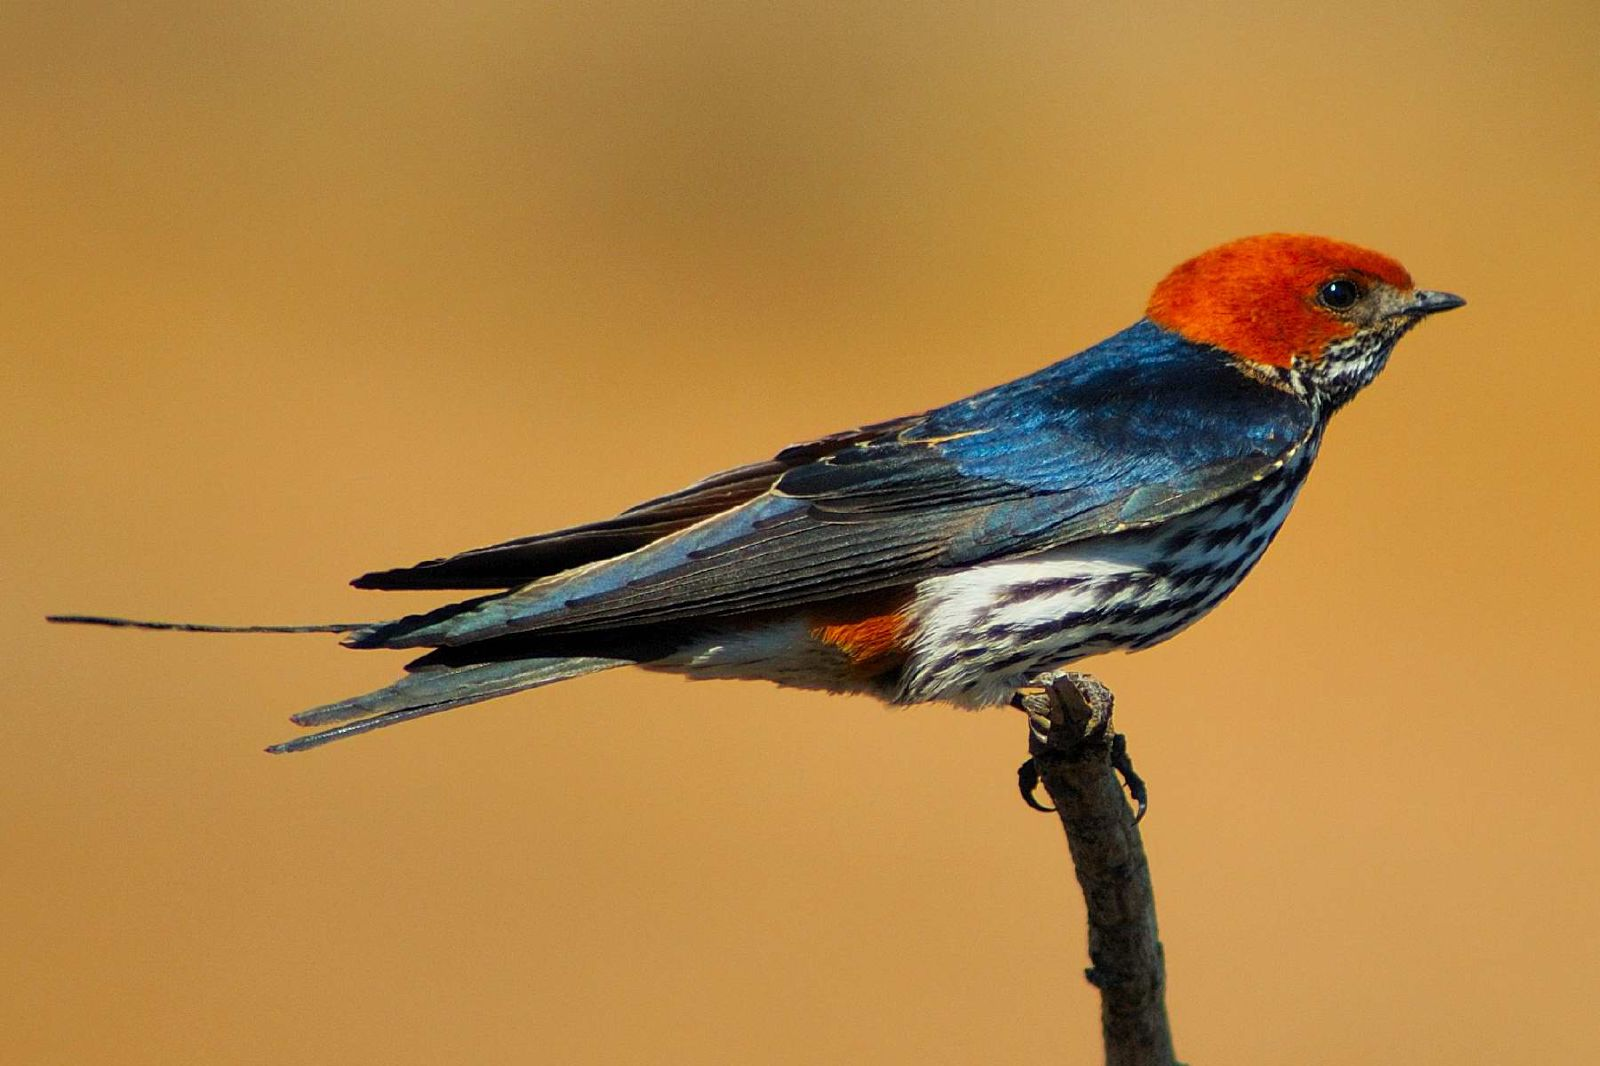
\includegraphics[width=0.5\columnwidth]{figures/swallow.jpg} % Example image
\end{center}

%------------------------------------------------

\subsection*{Answer}

While this question leaves out the crucial element of the geographic origin of the swallow, according to Jonathan Corum, an unladen European swallow maintains a cruising airspeed velocity of \textbf{11 metres per second}, or \textbf{24 miles an hour}. The velocity of the corresponding African swallows requires further research as kinematic data is severely lacking for these species.

%----------------------------------------------------------------------------------------

\ctikzfig{fig1}
\ctikzfig{fig3}
\ctikzfig{fig4}
\ctikzfig{fig5}
\ctikzfig{fig6}
\ctikzfig{fig7}
\section*{Question 2}

\begin{problem}
	How much wood would a woodchuck chuck if a woodchuck could chuck wood?
	
	\medskip
	
	\begin{enumerate}[(\itshape a\normalfont)] % Sub-questions styled as italic letters
		\item Suppose ``chuck" implies throwing.
		\item Suppose ``chuck" implies vomiting.
	\end{enumerate}
\end{problem}

%------------------------------------------------

\subsection*{Answer}

\begin{enumerate}[(\itshape a\normalfont)] % Sub-questions styled as italic letters
	\item According to the Associated Press (1988), a New York Fish and Wildlife technician named Richard Thomas calculated the volume of dirt in a typical 25--30 foot (7.6--9.1 m) long woodchuck burrow and had determined that if the woodchuck had moved an equivalent volume of wood, it could move ``about \textbf{700 pounds (320 kg)} on a good day, with the wind at his back".
    
	\item A woodchuck can ingest 361.92 cm\textsuperscript{3} (22.09 cu in) of wood per day. Assuming immediate expulsion on ingestion with a 5\% retainment rate, a woodchuck could chuck \textbf{343.82 cm\textsuperscript{3}} of wood per day.
\end{enumerate}

%----------------------------------------------------------------------------------------

\section*{Esercizio 3}

\begin{problem}
	\smallskip
	Mary is in prison and has 3 dollars; she can get out on bail if he
	has 8 dollars. A guard agrees to make a series of bets with her.
	If Mary bets A dollars, she wins A dollars with probability 0.4 and loses A dollars with probability 0.6.
	Find the probability that she wins 8 dollars before losing all of his money if
	\medskip
	\begin{enumerate}[(\itshape a\normalfont)]
		\item she bets 1 dollar each time (timid strategy).
		\item she bets, each time, as much as possible but not more than necessary to bring his fortune up to 8 dollars (bold strategy).
	\end{enumerate}
	\smallskip
	Which strategy gives Mary the better chance of getting out of jail?
	\smallskip
\end{problem}

%------------------------------------------------

\subsection*{Soluzione}

\begin{enumerate}[(\itshape a\normalfont)]
	\item La strategia timida definisce una DTMC le cui probabilità di transizione sono date da:
		\begin{equation*}
			\begin{aligned}
				&\mathbb{P}(0, 0) = 1,	\\
				&\mathbb{P}(i, i+1) = p = 0.4	\qquad &i = 1, \dots, 7,	\\
				&\mathbb{P}(i, i-1) = q = 1-p = 0.6	\qquad &i = 1, \dots, 7,	\\
				&\mathbb{P}(8, 8) = 1.
			\end{aligned}
		\end{equation*}
		Mentre il rispettivo grafo è dato da
		\ctikzfig{fig4}
		Ponendoci nel caso generale, supponiamo di partire con $0 \leq n \leq 8$ dollari.
		Sia $U_n$ l'evento "uscire dalla prigione partendo con n dollari", $V$ l'evento "Mary vince una scommessa" e $P = \overline{V}$ "Mary perde una scommessa".
		Allora, per la formula delle probabilità assoluta si ha che
		\begin{equation} \label{eq:es3_1}
			\begin{aligned}
				\mathbb{P}(U_n) &= \mathbb{P}(U_n | V)\mathbb{P}(V) + \mathbb{P}(U_n | P)\mathbb{P}(P) \\
					&= \mathbb{P}(U_n | V)p + \mathbb{P}(U_n | P)q \\
					&= \mathbb{P}(U_{n+1})p + \mathbb{P}(U_{n-1}) q.
			\end{aligned}
		\end{equation}
		L'ultima uguaglianza segue dal fatto che, sapendo di aver vinto una scommessa, avrò $n+1$ dollari, per cui $\mathbb{P}(U_n | V) = \mathbb{P}(U_{n+1})$.
		Possiamo effettuare un ragionamento simile nel caso in cui Mary perda una scommessa.
		Definiamo ora per semplicità di notazione $u_n = \mathbb{P}(U_n)$.
		Otteniamo così l'equazione ricorsiva con condizioni al contorno su $u_0, u_8$:
		\begin{equation*}
			\begin{cases}
				u_n = u_{n+1}p + u_{n-1}q \qquad n = 1, \dots, 7, \\
				u_0 = 0, \\
				u_8 = 1.
			\end{cases}
		\end{equation*}
		Possiamo risolvere tale equazione ricorsiva lineare del secondo ordine risolvendo prima l'equazione associata
		\begin{equation*}
			px^2 - x + q = 0.
		\end{equation*}
		Da cui si ricavano le soluzioni
		\begin{align*}
			x_1 &= \frac{1 + \sqrt{1 - 4pq}}{2p}, & x_2 &= \frac{1 - \sqrt{1 - 4pq}}{2p}.
		\end{align*}
		Ponendo $p = 0.4$, e quindi $q = 0.6$, si ottiene $x_1 = \frac{3}{2}$, $x_2 = 1$.
		Dunque si ha che
		\begin{equation*}
			u_n = Ax_1^n + Bu_2^n = A\left( \frac{3}{2} \right)^n + B,
		\end{equation*}
		dove $A$ e $B$ sono costanti che si ottengono applicando le condizioni al contorno
		\begin{equation*}
			\begin{gathered}
				u_0 = 0 = A + B \Rightarrow  B = -A, \\
				u_8 = 1 = A\left( \left( \frac{3}{2} \right)^8 - 1 \right) \Rightarrow A = - \frac{1}{\left( \frac{3}{2} \right)^8 - 1}.
			\end{gathered}
		\end{equation*}
		In conclusione, vale che
		\begin{equation*}
			u_n = \frac{\left( \frac{3}{2} \right)^n - 1}{\left( \frac{3}{2} \right)^8 - 1},
		\end{equation*}
		ed in particolare, ponendo $n = 3$, si ottiene che $u_3 \approx 0.0964$.
	
	\item La strategia audace consiste invece nel scommettere ad ogni passo una quantità data da $min\{n, 8-n\}$.
		In questo modo, l'\autoref{eq:es3_1} diventa:
		\begin{equation*}
			u_n = u_{min\{2n, 8\}}p + u_{max\{0, 2n-8\}}q.
		\end{equation*}
		Partendo dal valore $n = 3$, e ricordando le condizioni iniziali $u_0 = 0, u_8 = 1$, si ricavano le seguenti equazioni:
		\begin{equation*}
			\begin{aligned}
				u_3 &= u_6p + u_0q = u_6p,	\\
				u_6 &= u_8p + u_4q = p + u_4q,	\\
				u_4 &= u_8p + u_0q = p.				
			\end{aligned}
		\end{equation*}
		Da cui, procedendo ricorsivamente e ponendo $p = 0.4$, si ottiene:
		\begin{equation*}
			u_3 = (p + pq)p = p^2(1 + q) = 0.256.
		\end{equation*}
\end{enumerate}
In conclusione, la strategia audace è più efficace.
In tal caso Mary ha una probabilità di uscire di prigione del $25.6\%$, contro il $9.64\%$ della strategia timida.
%----------------------------------------------------------------------------------------

\section*{Esercizio 4}

\begin{problem}
	\smallskip
	Consider a DTMC with state space $S = \{0,...,N\}$ and transition probabilities $p(i, i+1) = p, p(i, i-1) = q$, for $1 \leq i \leq N$ where $p+q =1, 0 < p < 1$; assume $p(0, 0) = p(N,N-1)= q$ and $p(0, 1) = p(N,N)= p$.
	\medskip
	\begin{enumerate}[(\itshape a\normalfont)]
		\item Draw the graph (= transition diagram).
		\item Is the Markov chain irreducible?
		\item Is it aperiodic?
		\item What is the period of the chain?
		\item Find the stationary distribution.
	\end{enumerate}
	\smallskip
\end{problem}

%------------------------------------------------

\subsection*{Soluzione}

\begin{enumerate}[(\itshape a\normalfont)]
	\item Il grafo definito dalla DTMC è dato da
		\ctikzfig{fig6}
		Notiamo che tale catena è un processo di nascita e morte definito sull'intervallo $0, \dots, N$.
	\item La catena è irriducibile. Infatti $\forall i,j \in S$, come si può vedere dal grafo, esiste un cammino che congiunge i due nodi, cioé $i \leftrightarrow j$.
	\item La catena è aperiodica. Per mostrarlo ricordiamo che il periodo è una proprietà di classe, e quindi siccome la catena è aperiodica è uguale per tutti gli stati in $S$.
		Prendiamo lo stato $i = 0$. Questo ha un self-loop, quindi è aperiodico e di conseguenza la DTMC stessa è aperiodica.
	\item La catena è aperiodica, quindi ha periodo unitario.
	\item La catena è finita e irriducibile, quindi esiste ed è unica la distribuzione stazionaria $\pi = (\pi(i))_{i \in S}$.
		Inoltre, in quanto è un processo di nascita e morte, segue che la catena stazionaria è anche reversibile.
		Da qui si può ricavare la distribuzione stazionaria definita da
		\begin{equation*}
			\pi(0) = \frac{1}{M},	\qquad\qquad	\pi(x) = \pi(0) \left( \prod_{i=0}^{x-1} \frac{p}{q} \right) = \pi(0) \left(\frac{p}{q}\right)^x,
		\end{equation*}
		dove
		\begin{equation*}
			M = \sum_{x=0}^N \prod_{i=0}^{x-1} \left( \frac{p}{q} \right) = \sum_{x=0}^N \left(\frac{p}{q}\right)^x.
		\end{equation*}
		
	
\end{enumerate}
%----------------------------------------------------------------------------------------

\section*{Question 5 (bonus marks)}

\begin{problem}
	\lstinputlisting[
		caption=Luftballons Perl Script, % Caption above the listing
		label=lst:luftballons, % Label for referencing this listing
		language=Perl, % Use Perl functions/syntax highlighting
		frame=single, % Frame around the code listing
		showstringspaces=false, % Don't put marks in string spaces
		numbers=left, % Line numbers on left
		numberstyle=\tiny, % Line numbers styling
	]{codes/luftballons.pl}
	
	\begin{enumerate}
		\item How many luftballons will be output by the Listing \ref{lst:luftballons} above?
		\item Identify the regular expression in Listing \ref{lst:luftballons} and explain how it relates to the anti-war sentiments found in the rest of the script.
	\end{enumerate}

\end{problem}

%------------------------------------------------

\subsection*{Answer}

\begin{enumerate}
	\item 99 luftballons.
	\item Lorem ipsum dolor sit amet, consectetur adipiscing elit. Praesent porttitor arcu luctus, imperdiet urna iaculis, mattis eros. Pellentesque iaculis odio vel nisl ullamcorper, nec faucibus ipsum molestie. Sed dictum nisl non aliquet porttitor. Etiam vulputate arcu dignissim, finibus sem et, viverra nisl. Aenean luctus congue massa, ut laoreet metus ornare in. Nunc fermentum nisi imperdiet lectus tincidunt vestibulum at ac elit. Nulla mattis nisl eu malesuada suscipit.
\end{enumerate}

%----------------------------------------------------------------------------------------

\end{document}
